\documentclass{beamer}
\usepackage{eurosym}
\usepackage{color}
\usepackage{xcolor}
\usepackage{graphicx}
\usepackage{tikz}
\usepackage{mdframed}
\usetikzlibrary{arrows, positioning, decorations.pathmorphing, patterns}
\usetheme{metropolis}

% title, names, ...
\date{\today}
\author{Lukas Westhofen \and Christoph Welzel}
\institute{ComSys, RWTH Aachen}
\title{Submarine \hspace{4.2cm}\parbox{4cm}{\resizebox{4cm}{!}{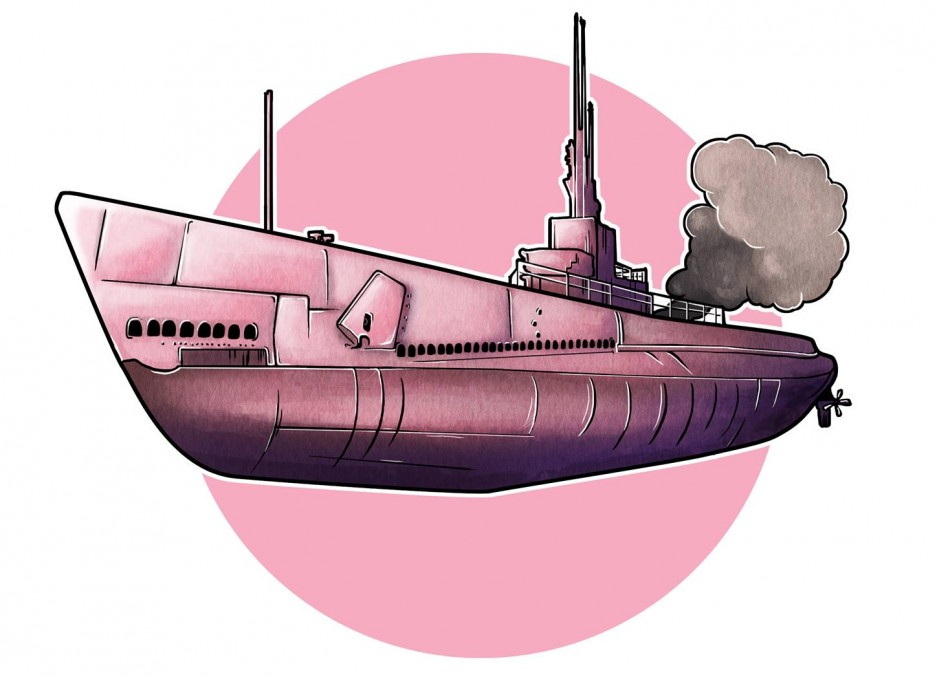
\includegraphics{pic/logo}}}}
\subtitle{Team Voltidioten}

% metropolis theme configuration
\definecolor{CorporateRose}{HTML}{F6ABC0}
\definecolor{DarkKhaki}{HTML}{BDB76B}
\definecolor{NavyBlue}{HTML}{000080}

\setbeamercolor{normal text}{bg=white, fg=black}
\setbeamercolor{progress bar}{bg=CorporateRose, fg=CorporateRose}
\setbeamercolor{title separator}{fg=CorporateRose, bg=CorporateRose}
\setbeamercolor{frametitle}{parent=structure, bg=CorporateRose}
\metroset{numbering=fraction}

\begin{document}

	\maketitle

	\section{Idea}
	\begin{frame}{Sketch: Concept}
		\begin{center}
			\resizebox{0.7\textwidth}{!}{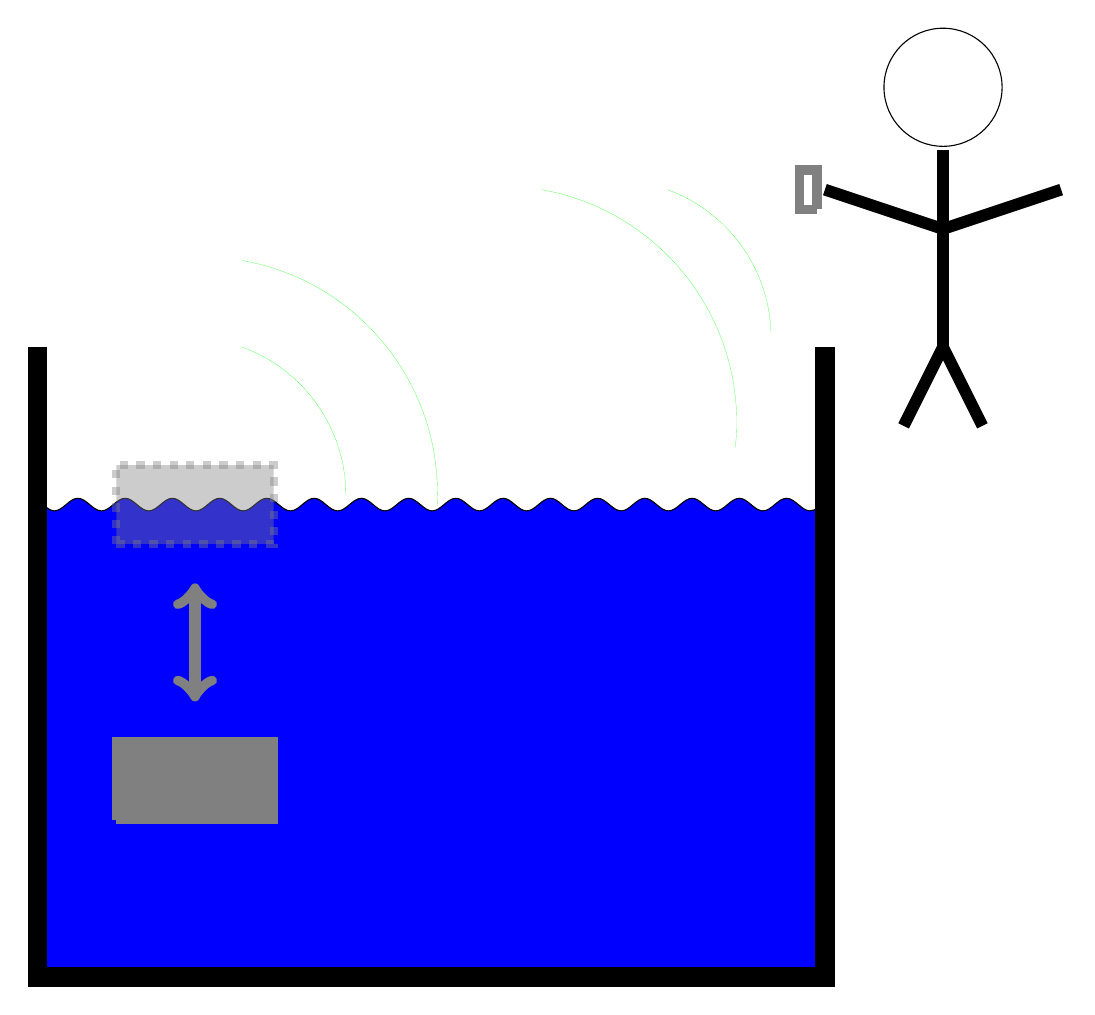
\begin{tikzpicture}
	\draw[
		decoration={
			snake,
			amplitude=0.8mm,
			segment length=6mm
		},
		fill=blue
	] decorate {(10,6) -- (0,6)} -- (0,0) -- (10,0) -- (10,6);
	\draw[
		line width=0.25cm
	] (10,8) -- (10,0) -- (0,0) -- (0,8);
	\draw[
		color=gray,
		fill=gray,
		line width=0.1cm
	] (1,2) -- (3,2) -- (3,3) -- (1,3) -- (1,2);
	\draw[
		color=black,
		line width=0.15cm
	] (11,7) -- (11.5,8) -- (12,7);
	\draw[
		color=black,
		line width=0.15cm
	] (11.5,8) -- (11.5,10.5);
	\draw[
		color=black,
		line width=0.15cm
	] (11.5, 9.5) -- (10, 10);
	\draw[
		color=black,
		line width=0.15cm
	] (11.5, 9.5) -- (13, 10);
	\node[
		circle,
		draw,
		minimum width=1.5cm,
		inner sep=0pt
	] (head) at (11.5, 11.3) {};
	\draw[
		color=gray,
		line width=0.12cm
	] (9.9,9.75) -- (9.9,10.25) -- (9.68,10.25) -- (9.68, 9.75) -- (9.9,9.75);
	\draw[
		color=gray,
		line width=0.1cm,
		fill=gray,
		opacity=0.4,
		dashed
	] (1,5.5) -- (3,5.5) -- (3,6.5) -- (1,6.5) -- (1,5.5);
	\draw[
		<->,
		line width=0.15cm,
		color=gray
	] (2,5) -- (2,3.5);
	\draw[
		color=green,
		line width=0.05
	] (2.6,8) arc (70:0:2cm);
	\draw[
		color=green,
		line width=0.05
	] (2.6,9.1) arc (80:-3:3cm);
	\draw[
		color=green,
		line width=0.05
	] (6.4,10) arc (80:-6:3cm);
	\draw[
		color=green,
		line width=0.05
	] (8,10) arc (70:2:2cm);


\end{tikzpicture}
}
		\end{center}
	\end{frame}

	\begin{frame}{Objectives}
		\begin{columns}
			\begin{column}{0.5\textwidth}
				\begin{itemize}
					\item low-cost, easy to build submarine
					\item autonomous dives
					\item data gathering
					\item data representation on device
				\end{itemize}
			\end{column}
			\begin{column}{0.5\textwidth}
				\begin{itemize}
					\item learning experience
					\item monitoring waters
					\item teaching project (students, pupils,\dots)
				\end{itemize}
			\end{column}
		\end{columns}
	\end{frame}

	\section{Submarine}

	\begin{frame}{Sketch: Submarine}
		\begin{center}
			\resizebox{\textwidth}{!}{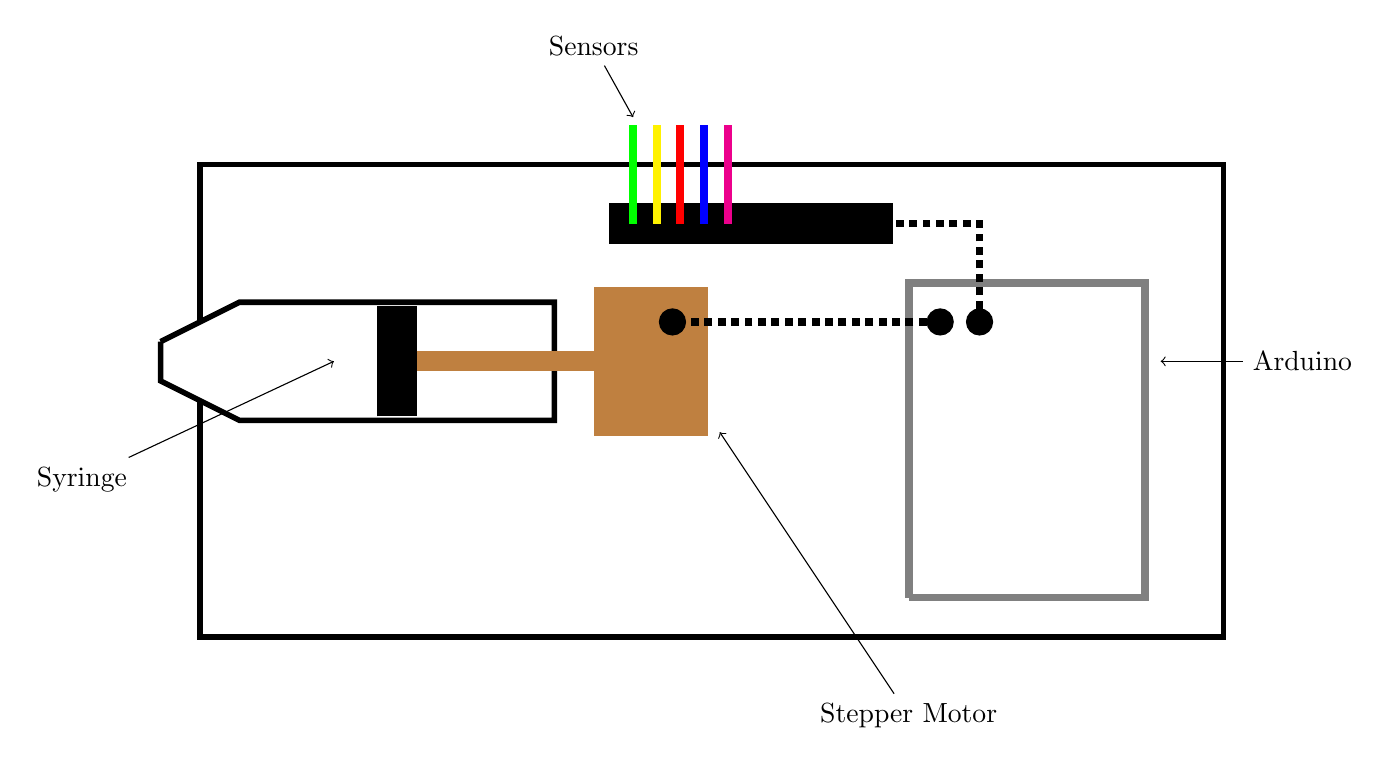
\begin{tikzpicture}
	% Hülle
	\draw[
		line width=0.07cm
	] (1,5) -- (1,2) -- (14,2) -- (14,8) -- (1,8) -- (1,6);
	% Spritze(oben)
	\draw[
		line width=0.07cm
	] (0.5,5.75) -- (0.5,5.25) -- (1.5,4.75) -- (5.5,4.75) -- (5.5,6.25) --
		(1.5,6.25) -- (0.5,5.75);
	% Arduino
	\draw[
		line width=0.1cm,
		color=gray
	] (10,2.5) -- (13,2.5) -- (13,6.5) -- (10,6.5) -- (10,2.5);
	% Servo(oben)
	\draw[
		line width=0.9cm,
		color=brown,
		fill=brown
	] (6,5) -- (7,5) -- (7,6) -- (6,6);
	% Kolben(oben)
	\draw[
		line width=0.5cm,
		color=black
	] (3.5,4.8) -- (3.5,6.2);
	% Verbindung Servo Kolben (oben)
	\draw[
		line width=0.25cm,
		color=brown
	] (3.75,5.5) -- (6,5.5);
	% Ansteuerung Servo (oben)
	\node[
		circle,
		draw,
		fill=black
	] at (10.4,6) {};
	\node[
		circle,
		draw,
		fill=black
	] at (7,6) {};
	\draw[
		dotted,
		color=black,
		line width=0.1cm
	] (10.4,6) -- (7,6);
	% Sensoren-Bank
	\draw[
		fill=black
	] (6.2,7) -- (9.8,7) -- (9.8,7.5) -- (6.2,7.5);
	% Sensoren
	\draw[
		color=green,
		line width=0.1cm
	] (6.5,7.25) -- (6.5,8.5);
	\draw[
		color=yellow,
		line width=0.1cm
	] (6.8,7.25) -- (6.8,8.5);
	\draw[
		color=red,
		line width=0.1cm
	] (7.1,7.25) -- (7.1,8.5);
	\draw[
		color=blue,
		line width=0.1cm
	] (7.4,7.25) -- (7.4,8.5);
	\draw[
		color=magenta,
		line width=0.1cm
	] (7.7,7.25) -- (7.7,8.5);
	% Sensoren Ansteuerung
	\node[
		circle,
		fill=black,
		draw
	] at (10.9,6) {};
	\draw[
		dotted,
		color=black,
		line width=0.1cm
	] (10.9,6) -- (10.9,7.25) -- (9.7,7.25);

	% Erläuterung
	%  Begriffe
	\node (spritzen) at (-0.5,4)  {Syringe};
	\node (sensoren) at (6,9.5)   {Sensors};
	\node (servos)   at (10,1) {Stepper Motor};
	\node (arduino)  at (15,5.5)  {Arduino};
	%  Pfeile
	\draw [->] (spritzen) to (2.7,5.5);
	\draw [->] (sensoren) to (6.5,8.6);
	\draw [->] (servos)   to (7.6,4.6);
	\draw [->] (arduino)  to (13.2,5.5);
\end{tikzpicture}
}
		\end{center}
	\end{frame}

	\begin{frame}[t]{Dive Tank I}
		\begin{columns}[T]
			\begin{column}{0.5\textwidth}
				\begin{minipage}{\textwidth}
					\resizebox{0.9\textwidth}{!}{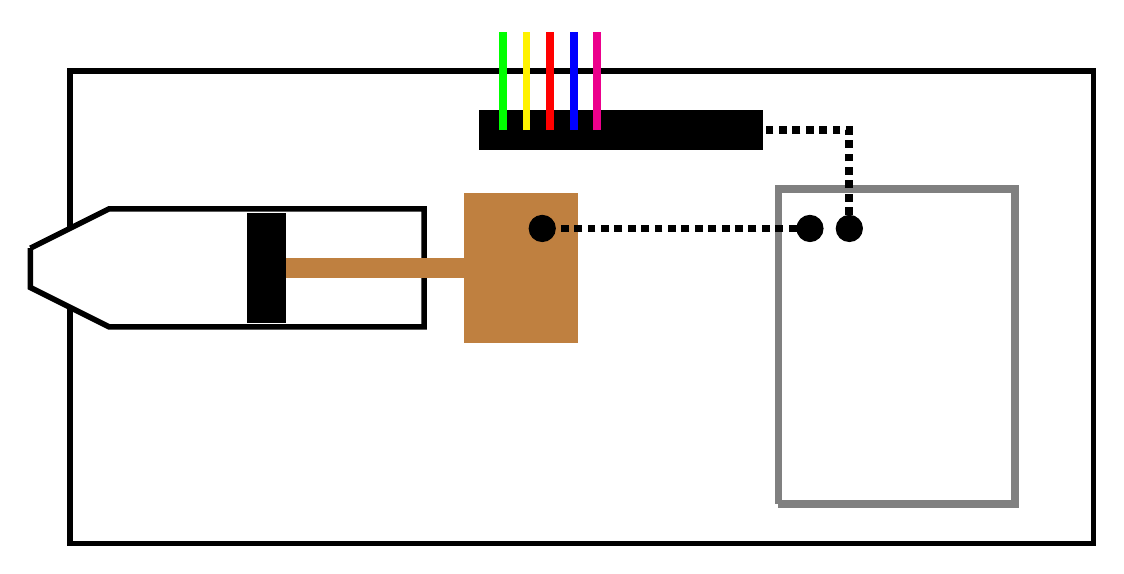
\begin{tikzpicture}
	% Hülle
	\draw[
		line width=0.07cm
	] (1,5) -- (1,2) -- (14,2) -- (14,8) -- (1,8) -- (1,6);
	% Spritze(oben)
	\draw[
		line width=0.07cm
	] (0.5,5.75) -- (0.5,5.25) -- (1.5,4.75) -- (5.5,4.75) -- (5.5,6.25) --
		(1.5,6.25) -- (0.5,5.75);
	% Arduino
	\draw[
		line width=0.1cm,
		color=gray
	] (10,2.5) -- (13,2.5) -- (13,6.5) -- (10,6.5) -- (10,2.5);
	% Servo(oben)
	\draw[
		line width=0.9cm,
		color=brown,
		fill=brown
	] (6,5) -- (7,5) -- (7,6) -- (6,6);
	% Kolben(oben)
	\draw[
		line width=0.5cm,
		color=black
	] (3.5,4.8) -- (3.5,6.2);
	% Verbindung Servo Kolben (oben)
	\draw[
		line width=0.25cm,
		color=brown
	] (3.75,5.5) -- (6,5.5);
	% Ansteuerung Servo (oben)
	\node[
		circle,
		draw,
		fill=black
	] at (10.4,6) {};
	\node[
		circle,
		draw,
		fill=black
	] at (7,6) {};
	\draw[
		dotted,
		color=black,
		line width=0.1cm
	] (10.4,6) -- (7,6);
	% Sensoren-Bank
	\draw[
		fill=black
	] (6.2,7) -- (9.8,7) -- (9.8,7.5) -- (6.2,7.5);
	% Sensoren
	\draw[
		color=green,
		line width=0.1cm
	] (6.5,7.25) -- (6.5,8.5);
	\draw[
		color=yellow,
		line width=0.1cm
	] (6.8,7.25) -- (6.8,8.5);
	\draw[
		color=red,
		line width=0.1cm
	] (7.1,7.25) -- (7.1,8.5);
	\draw[
		color=blue,
		line width=0.1cm
	] (7.4,7.25) -- (7.4,8.5);
	\draw[
		color=magenta,
		line width=0.1cm
	] (7.7,7.25) -- (7.7,8.5);
	% Sensoren Ansteuerung
	\node[
		circle,
		fill=black,
		draw
	] at (10.9,6) {};
	\draw[
		dotted,
		color=black,
		line width=0.1cm
	] (10.9,6) -- (10.9,7.25) -- (9.7,7.25);

\end{tikzpicture}
}
				\end{minipage}
				\begin{minipage}{\textwidth}
					\vspace{0.5cm}
					\begin{itemize}
						\item countersink nut into plunger
						\item translate rotation of threaded rod to lifting motion
						\item[$\Rightarrow$] compact design\uncover<2>{,\textcolor{red}{ but unfortunatly leaky}}
					\end{itemize}
				\end{minipage}
			\end{column}
			\begin{column}{0.5\textwidth}
				\begin{center}
					\resizebox{0.5\textwidth}{!}{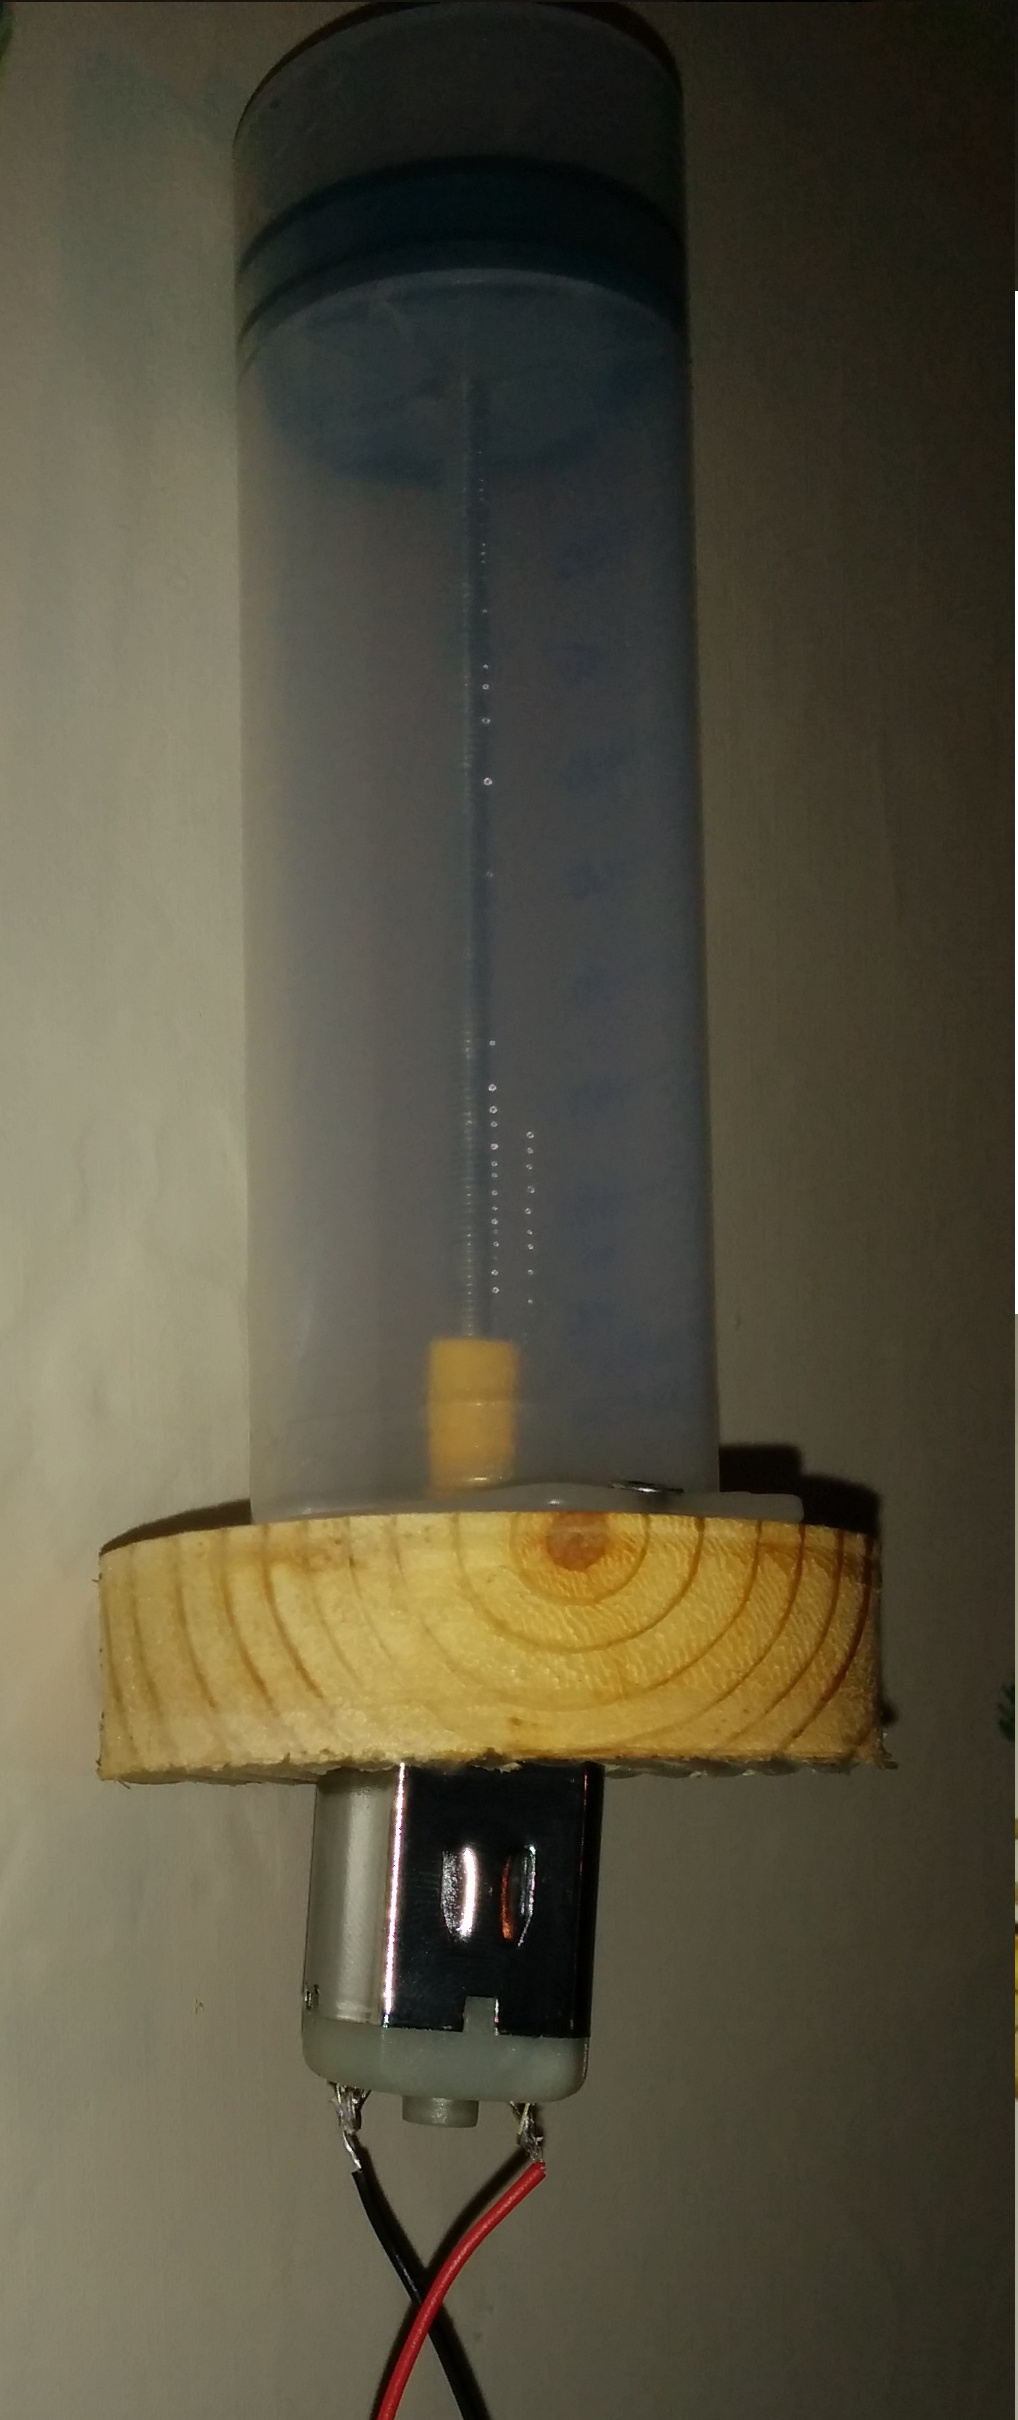
\includegraphics{pic/first-divetank}}
				\end{center}
			\end{column}
		\end{columns}
	\end{frame}

	\begin{frame}[t]{Dive Tank II}
		\begin{columns}[T]
			\begin{column}{0.5\textwidth}
				\begin{minipage}{\textwidth}
					\resizebox{0.9\textwidth}{!}{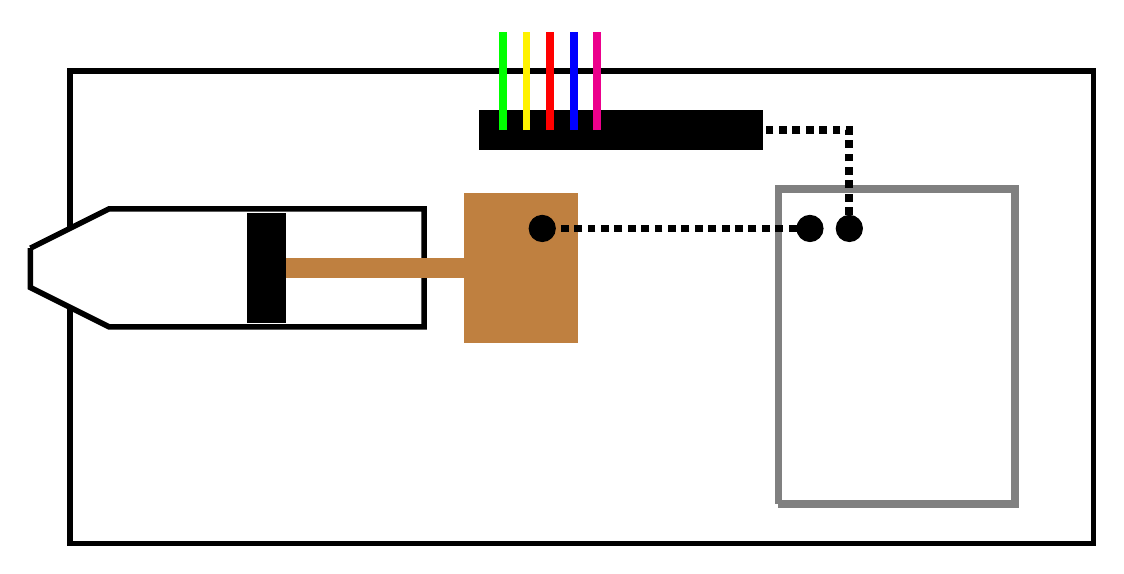
\begin{tikzpicture}
	% Hülle
	\draw[
		line width=0.07cm
	] (1,5) -- (1,2) -- (14,2) -- (14,8) -- (1,8) -- (1,6);
	% Spritze(oben)
	\draw[
		line width=0.07cm
	] (0.5,5.75) -- (0.5,5.25) -- (1.5,4.75) -- (5.5,4.75) -- (5.5,6.25) --
		(1.5,6.25) -- (0.5,5.75);
	% Arduino
	\draw[
		line width=0.1cm,
		color=gray
	] (10,2.5) -- (13,2.5) -- (13,6.5) -- (10,6.5) -- (10,2.5);
	% Servo(oben)
	\draw[
		line width=0.9cm,
		color=brown,
		fill=brown
	] (6,5) -- (7,5) -- (7,6) -- (6,6);
	% Kolben(oben)
	\draw[
		line width=0.5cm,
		color=black
	] (3.5,4.8) -- (3.5,6.2);
	% Verbindung Servo Kolben (oben)
	\draw[
		line width=0.25cm,
		color=brown
	] (3.75,5.5) -- (6,5.5);
	% Ansteuerung Servo (oben)
	\node[
		circle,
		draw,
		fill=black
	] at (10.4,6) {};
	\node[
		circle,
		draw,
		fill=black
	] at (7,6) {};
	\draw[
		dotted,
		color=black,
		line width=0.1cm
	] (10.4,6) -- (7,6);
	% Sensoren-Bank
	\draw[
		fill=black
	] (6.2,7) -- (9.8,7) -- (9.8,7.5) -- (6.2,7.5);
	% Sensoren
	\draw[
		color=green,
		line width=0.1cm
	] (6.5,7.25) -- (6.5,8.5);
	\draw[
		color=yellow,
		line width=0.1cm
	] (6.8,7.25) -- (6.8,8.5);
	\draw[
		color=red,
		line width=0.1cm
	] (7.1,7.25) -- (7.1,8.5);
	\draw[
		color=blue,
		line width=0.1cm
	] (7.4,7.25) -- (7.4,8.5);
	\draw[
		color=magenta,
		line width=0.1cm
	] (7.7,7.25) -- (7.7,8.5);
	% Sensoren Ansteuerung
	\node[
		circle,
		fill=black,
		draw
	] at (10.9,6) {};
	\draw[
		dotted,
		color=black,
		line width=0.1cm
	] (10.9,6) -- (10.9,7.25) -- (9.7,7.25);

\end{tikzpicture}
}
				\end{minipage}
				\begin{minipage}{\textwidth}
					\vspace{0.5cm}
					\begin{itemize}
						\item move nut to end of plunger
							\begin{itemize}
								\item[$\Rightarrow$] leave seal intact
							\end{itemize}
						\item not as compact\uncover<2>{, but leak-free}
					\end{itemize}
				\end{minipage}
			\end{column}
			\begin{column}{0.5\textwidth}
				\begin{center}
					\resizebox{0.37\textwidth}{!}{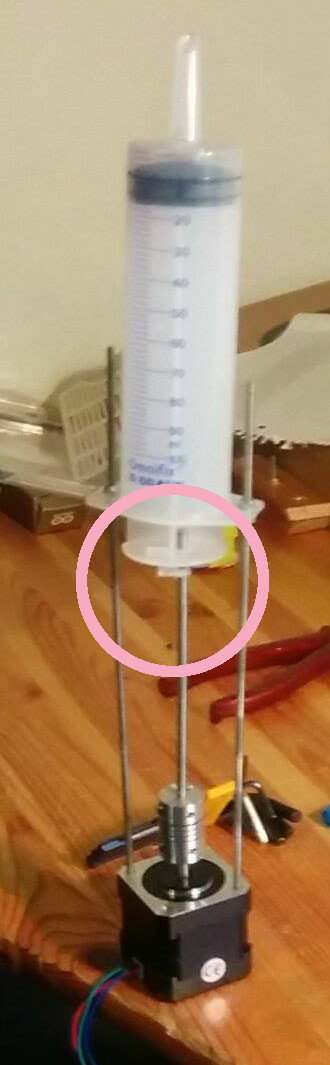
\includegraphics{pic/second-divetank}}
				\end{center}
			\end{column}
		\end{columns}
	\end{frame}

	\begin{frame}[t]{Sensors}
		\begin{columns}[T]
			\begin{column}{0.5\textwidth}
				\begin{minipage}{\textwidth}
					\resizebox{0.9\textwidth}{!}{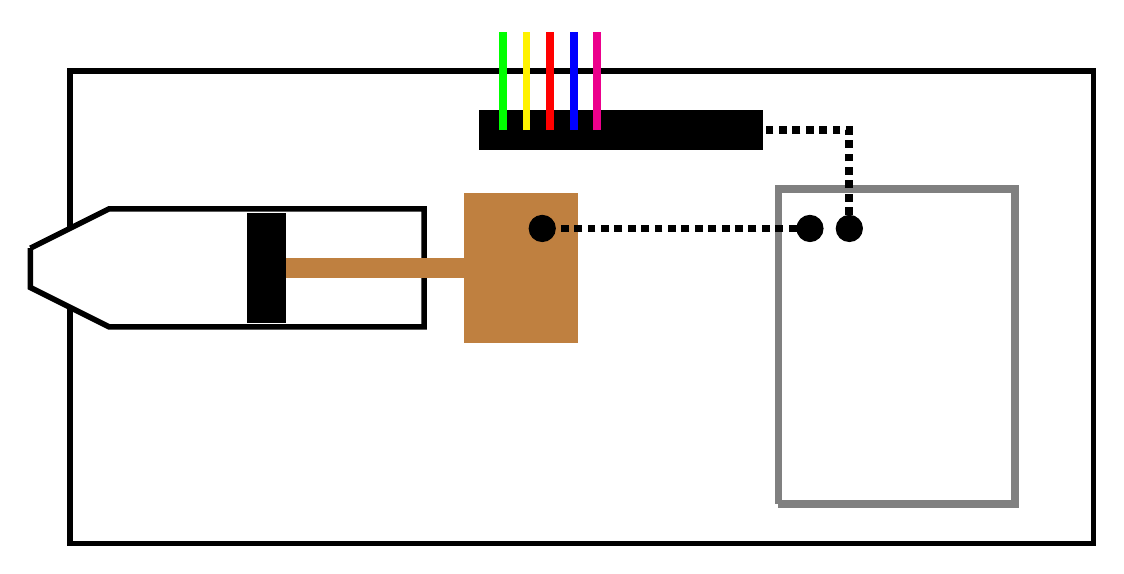
\begin{tikzpicture}
	% Hülle
	\draw[
		line width=0.07cm
	] (1,5) -- (1,2) -- (14,2) -- (14,8) -- (1,8) -- (1,6);
	% Spritze(oben)
	\draw[
		line width=0.07cm
	] (0.5,5.75) -- (0.5,5.25) -- (1.5,4.75) -- (5.5,4.75) -- (5.5,6.25) --
		(1.5,6.25) -- (0.5,5.75);
	% Arduino
	\draw[
		line width=0.1cm,
		color=gray
	] (10,2.5) -- (13,2.5) -- (13,6.5) -- (10,6.5) -- (10,2.5);
	% Servo(oben)
	\draw[
		line width=0.9cm,
		color=brown,
		fill=brown
	] (6,5) -- (7,5) -- (7,6) -- (6,6);
	% Kolben(oben)
	\draw[
		line width=0.5cm,
		color=black
	] (3.5,4.8) -- (3.5,6.2);
	% Verbindung Servo Kolben (oben)
	\draw[
		line width=0.25cm,
		color=brown
	] (3.75,5.5) -- (6,5.5);
	% Ansteuerung Servo (oben)
	\node[
		circle,
		draw,
		fill=black
	] at (10.4,6) {};
	\node[
		circle,
		draw,
		fill=black
	] at (7,6) {};
	\draw[
		dotted,
		color=black,
		line width=0.1cm
	] (10.4,6) -- (7,6);
	% Sensoren-Bank
	\draw[
		fill=black
	] (6.2,7) -- (9.8,7) -- (9.8,7.5) -- (6.2,7.5);
	% Sensoren
	\draw[
		color=green,
		line width=0.1cm
	] (6.5,7.25) -- (6.5,8.5);
	\draw[
		color=yellow,
		line width=0.1cm
	] (6.8,7.25) -- (6.8,8.5);
	\draw[
		color=red,
		line width=0.1cm
	] (7.1,7.25) -- (7.1,8.5);
	\draw[
		color=blue,
		line width=0.1cm
	] (7.4,7.25) -- (7.4,8.5);
	\draw[
		color=magenta,
		line width=0.1cm
	] (7.7,7.25) -- (7.7,8.5);
	% Sensoren Ansteuerung
	\node[
		circle,
		fill=black,
		draw
	] at (10.9,6) {};
	\draw[
		dotted,
		color=black,
		line width=0.1cm
	] (10.9,6) -- (10.9,7.25) -- (9.7,7.25);

\end{tikzpicture}
}
				\end{minipage}
				\begin{minipage}{\textwidth}
					\vspace{0.5cm}
					\begin{itemize}
						\item pressure
							\begin{itemize}
								\item correlates with depth
								\item[$\Rightarrow$] can be used as reference quantity
							\end{itemize}
						\item temperature
						\item there are many more pins available\dots
					\end{itemize}
				\end{minipage}
			\end{column}
			\begin{column}{0.5\textwidth}
				\resizebox{0.8\textwidth}{!}{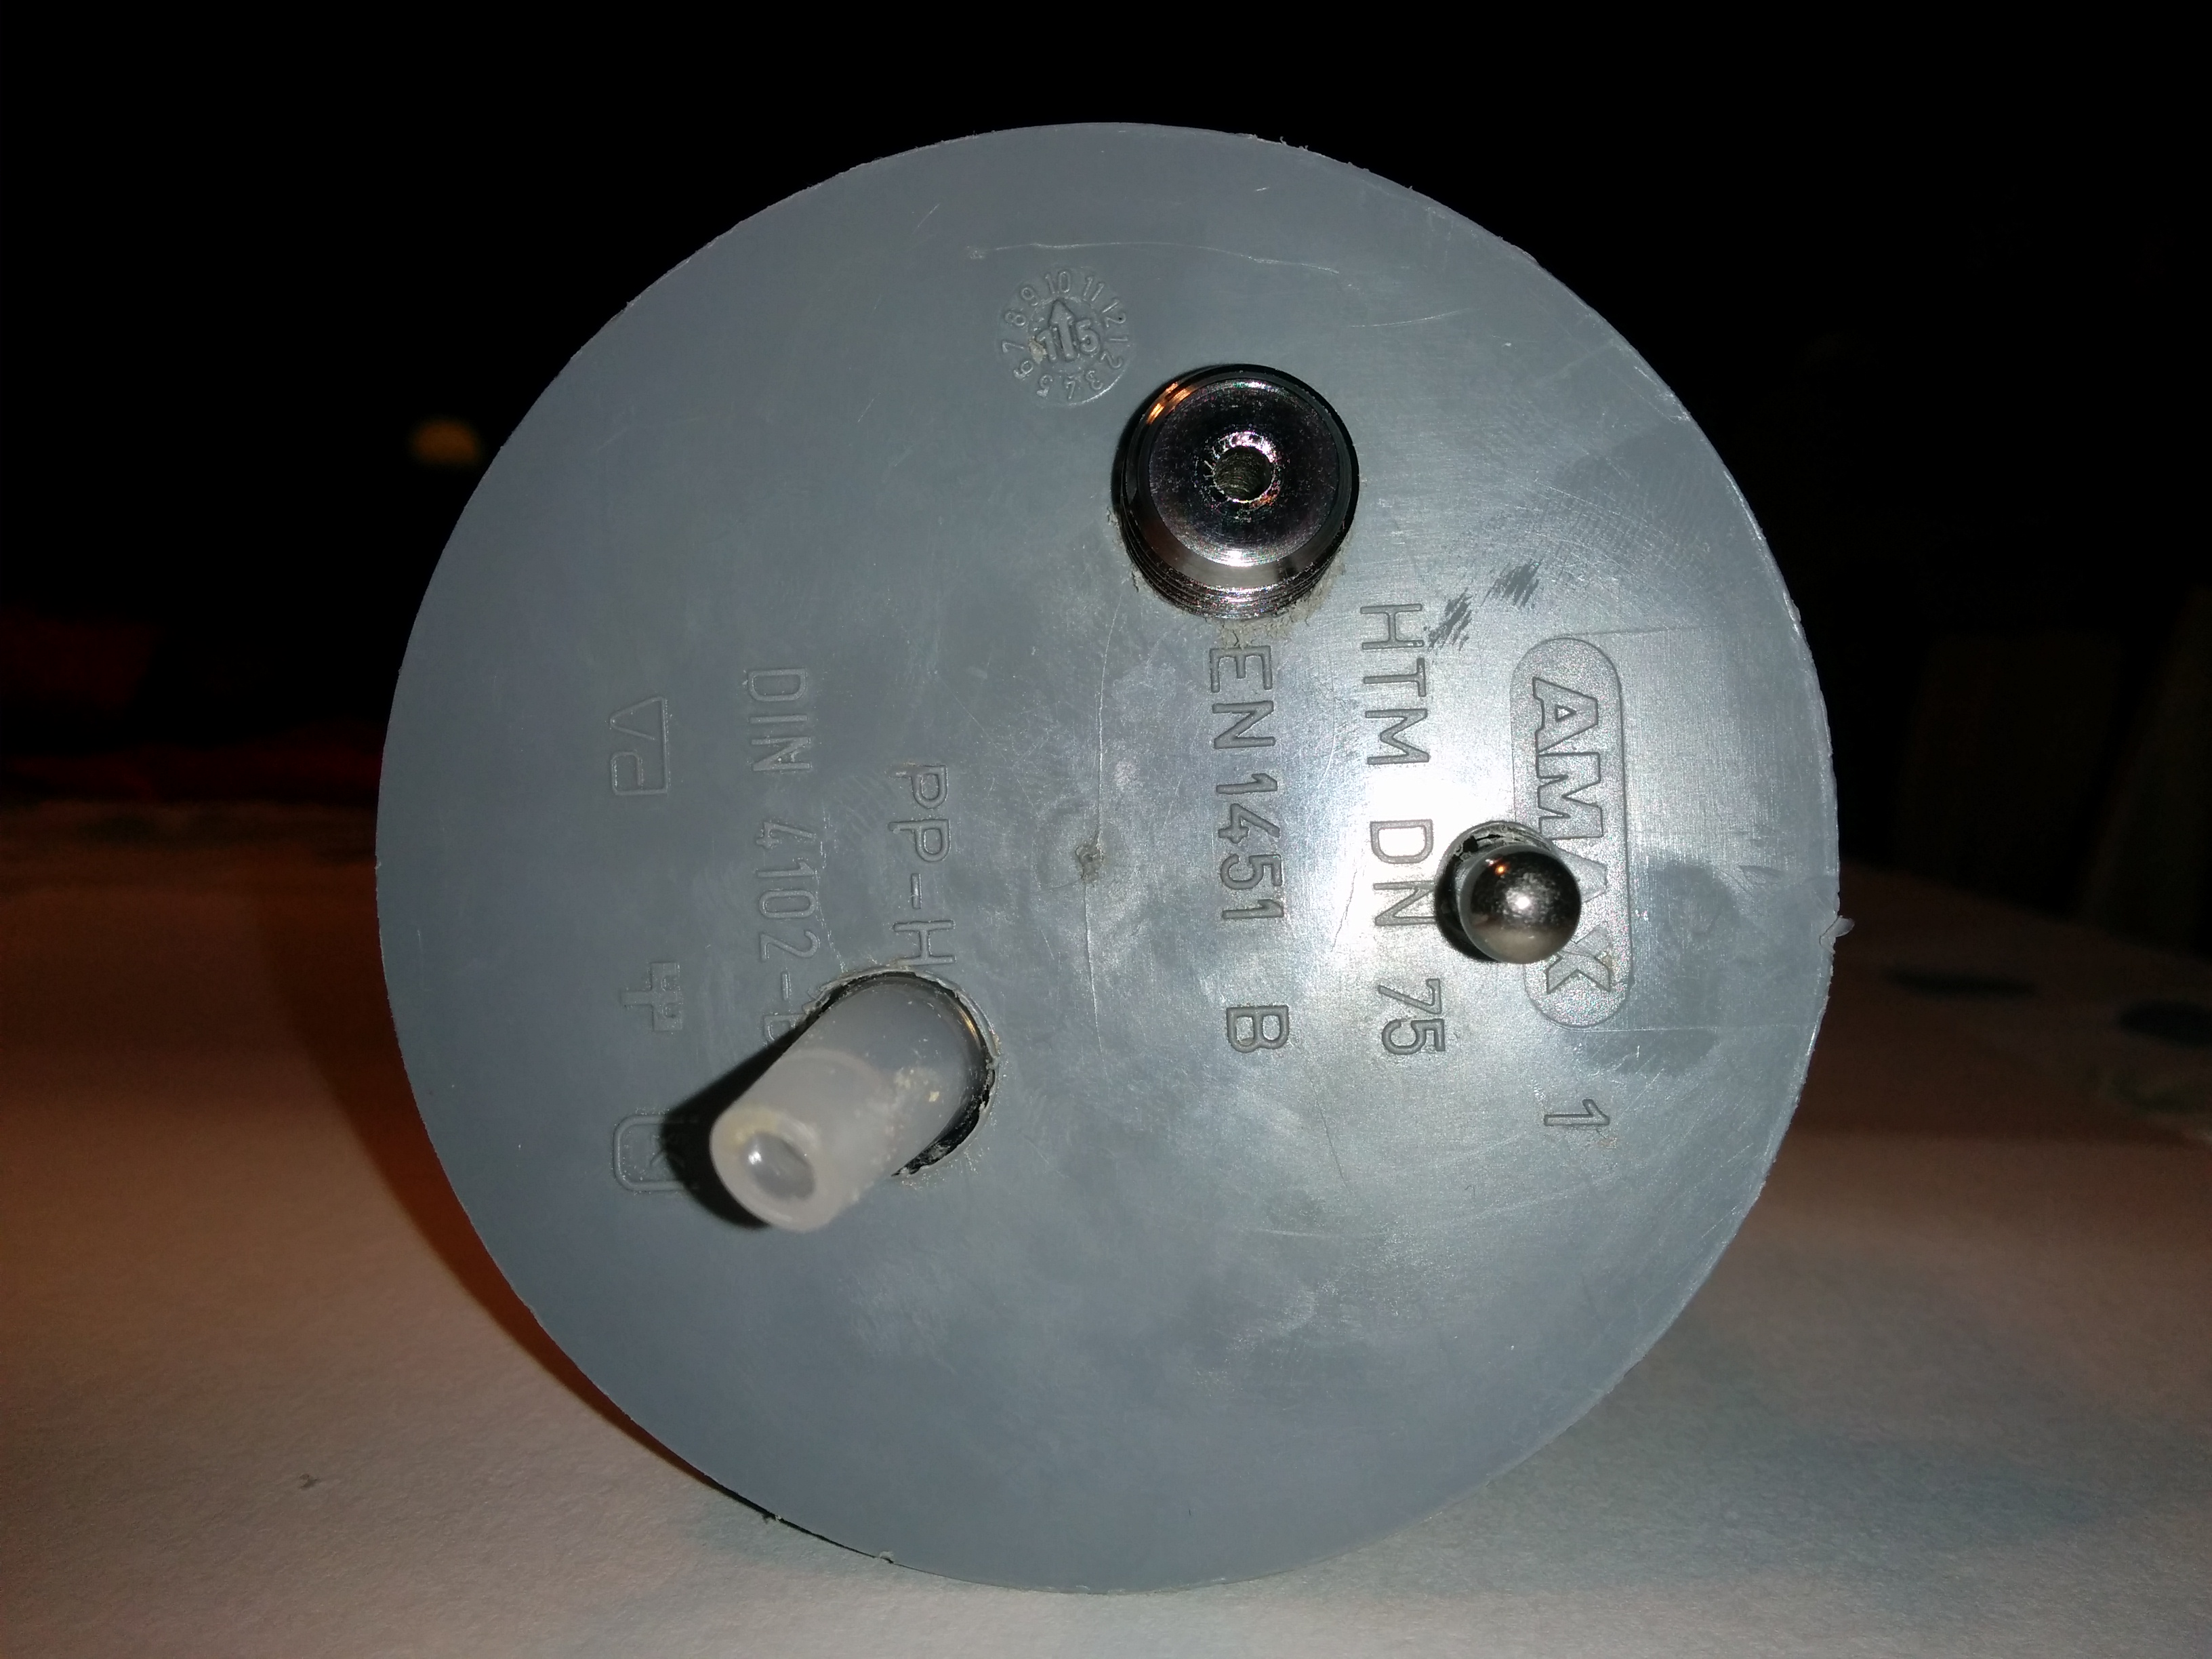
\includegraphics{pic/sensors-front}}
				\resizebox{0.8\textwidth}{!}{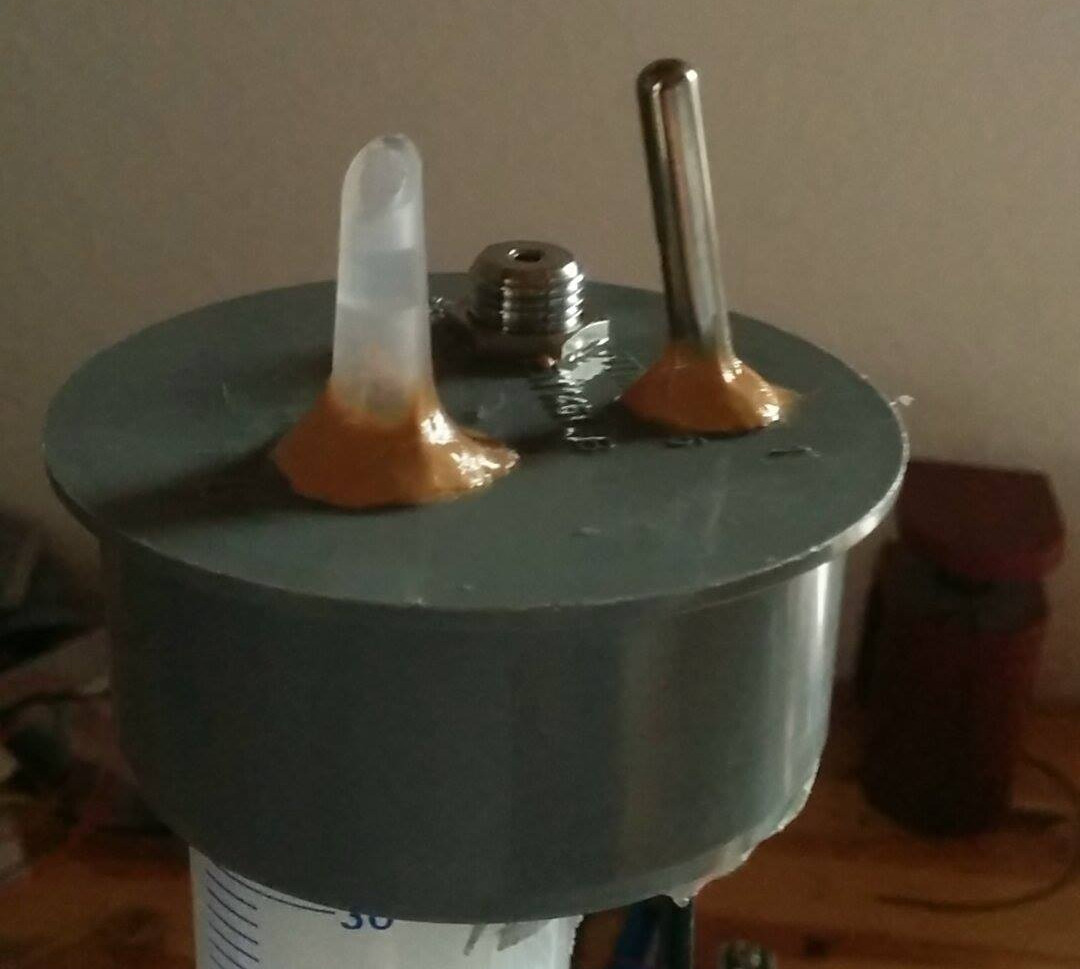
\includegraphics{pic/sensors-side}}
			\end{column}
		\end{columns}
	\end{frame}

	\begin{frame}[t]{Bluetooth Module}
		\begin{columns}[T]
			\begin{column}{0.5\textwidth}
				\begin{minipage}{\textwidth}
					\resizebox{0.9\textwidth}{!}{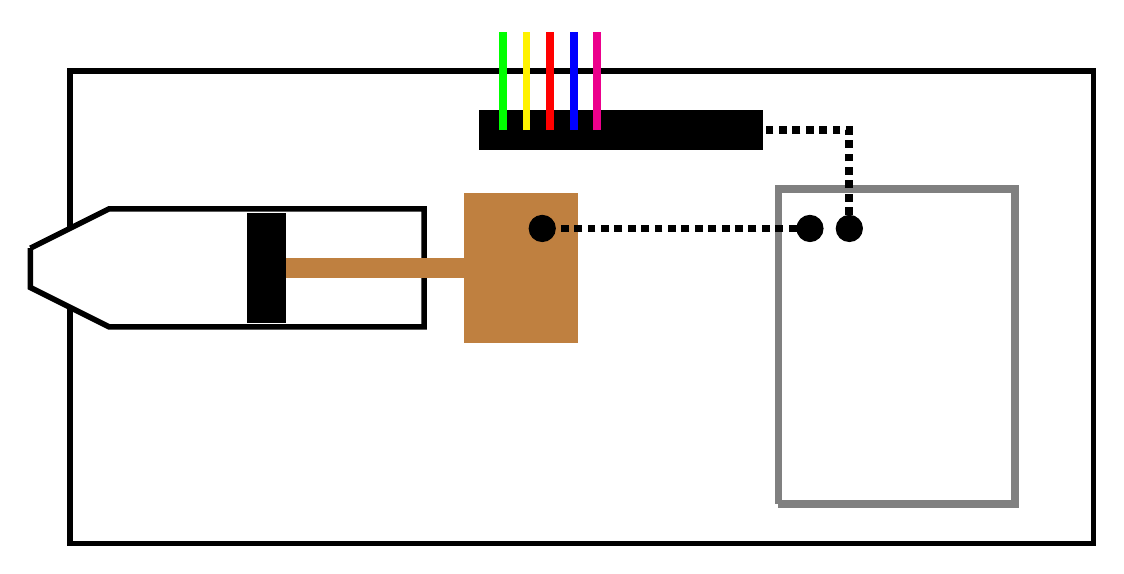
\begin{tikzpicture}
	% Hülle
	\draw[
		line width=0.07cm
	] (1,5) -- (1,2) -- (14,2) -- (14,8) -- (1,8) -- (1,6);
	% Spritze(oben)
	\draw[
		line width=0.07cm
	] (0.5,5.75) -- (0.5,5.25) -- (1.5,4.75) -- (5.5,4.75) -- (5.5,6.25) --
		(1.5,6.25) -- (0.5,5.75);
	% Arduino
	\draw[
		line width=0.1cm,
		color=gray
	] (10,2.5) -- (13,2.5) -- (13,6.5) -- (10,6.5) -- (10,2.5);
	% Servo(oben)
	\draw[
		line width=0.9cm,
		color=brown,
		fill=brown
	] (6,5) -- (7,5) -- (7,6) -- (6,6);
	% Kolben(oben)
	\draw[
		line width=0.5cm,
		color=black
	] (3.5,4.8) -- (3.5,6.2);
	% Verbindung Servo Kolben (oben)
	\draw[
		line width=0.25cm,
		color=brown
	] (3.75,5.5) -- (6,5.5);
	% Ansteuerung Servo (oben)
	\node[
		circle,
		draw,
		fill=black
	] at (10.4,6) {};
	\node[
		circle,
		draw,
		fill=black
	] at (7,6) {};
	\draw[
		dotted,
		color=black,
		line width=0.1cm
	] (10.4,6) -- (7,6);
	% Sensoren-Bank
	\draw[
		fill=black
	] (6.2,7) -- (9.8,7) -- (9.8,7.5) -- (6.2,7.5);
	% Sensoren
	\draw[
		color=green,
		line width=0.1cm
	] (6.5,7.25) -- (6.5,8.5);
	\draw[
		color=yellow,
		line width=0.1cm
	] (6.8,7.25) -- (6.8,8.5);
	\draw[
		color=red,
		line width=0.1cm
	] (7.1,7.25) -- (7.1,8.5);
	\draw[
		color=blue,
		line width=0.1cm
	] (7.4,7.25) -- (7.4,8.5);
	\draw[
		color=magenta,
		line width=0.1cm
	] (7.7,7.25) -- (7.7,8.5);
	% Sensoren Ansteuerung
	\node[
		circle,
		fill=black,
		draw
	] at (10.9,6) {};
	\draw[
		dotted,
		color=black,
		line width=0.1cm
	] (10.9,6) -- (10.9,7.25) -- (9.7,7.25);

\end{tikzpicture}
}
				\end{minipage}
				\begin{minipage}{\textwidth}
					\vspace{0.5cm}
					\begin{itemize}
						\item operates on 5 or 3.3 volts
						\item hardware driver
							\begin{itemize}
								\item easy to use for arduino
								\item communication via serial ports
							\end{itemize}
					\end{itemize}
				\end{minipage}
			\end{column}
			\begin{column}{0.5\textwidth}
				\resizebox{0.8\textwidth}{!}{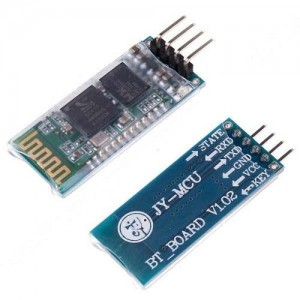
\includegraphics{pic/bluetooth-module}}
			\end{column}
		\end{columns}
	\end{frame}
	\begin{frame}[t]{Arduino}
		\begin{columns}[T]
			\begin{column}{0.5\textwidth}
				\begin{minipage}{\textwidth}
					\resizebox{0.9\textwidth}{!}{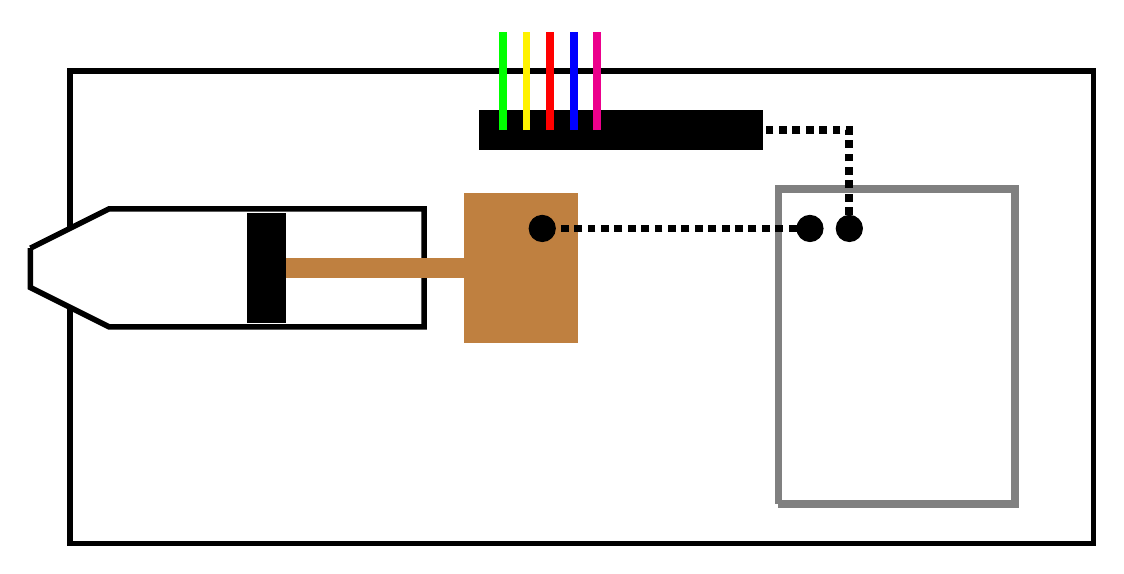
\begin{tikzpicture}
	% Hülle
	\draw[
		line width=0.07cm
	] (1,5) -- (1,2) -- (14,2) -- (14,8) -- (1,8) -- (1,6);
	% Spritze(oben)
	\draw[
		line width=0.07cm
	] (0.5,5.75) -- (0.5,5.25) -- (1.5,4.75) -- (5.5,4.75) -- (5.5,6.25) --
		(1.5,6.25) -- (0.5,5.75);
	% Arduino
	\draw[
		line width=0.1cm,
		color=gray
	] (10,2.5) -- (13,2.5) -- (13,6.5) -- (10,6.5) -- (10,2.5);
	% Servo(oben)
	\draw[
		line width=0.9cm,
		color=brown,
		fill=brown
	] (6,5) -- (7,5) -- (7,6) -- (6,6);
	% Kolben(oben)
	\draw[
		line width=0.5cm,
		color=black
	] (3.5,4.8) -- (3.5,6.2);
	% Verbindung Servo Kolben (oben)
	\draw[
		line width=0.25cm,
		color=brown
	] (3.75,5.5) -- (6,5.5);
	% Ansteuerung Servo (oben)
	\node[
		circle,
		draw,
		fill=black
	] at (10.4,6) {};
	\node[
		circle,
		draw,
		fill=black
	] at (7,6) {};
	\draw[
		dotted,
		color=black,
		line width=0.1cm
	] (10.4,6) -- (7,6);
	% Sensoren-Bank
	\draw[
		fill=black
	] (6.2,7) -- (9.8,7) -- (9.8,7.5) -- (6.2,7.5);
	% Sensoren
	\draw[
		color=green,
		line width=0.1cm
	] (6.5,7.25) -- (6.5,8.5);
	\draw[
		color=yellow,
		line width=0.1cm
	] (6.8,7.25) -- (6.8,8.5);
	\draw[
		color=red,
		line width=0.1cm
	] (7.1,7.25) -- (7.1,8.5);
	\draw[
		color=blue,
		line width=0.1cm
	] (7.4,7.25) -- (7.4,8.5);
	\draw[
		color=magenta,
		line width=0.1cm
	] (7.7,7.25) -- (7.7,8.5);
	% Sensoren Ansteuerung
	\node[
		circle,
		fill=black,
		draw
	] at (10.9,6) {};
	\draw[
		dotted,
		color=black,
		line width=0.1cm
	] (10.9,6) -- (10.9,7.25) -- (9.7,7.25);

\end{tikzpicture}
}
				\end{minipage}
				\begin{minipage}{\textwidth}
					\vspace{0.5cm}
					\begin{itemize}
						\item Arduino Uno
							\begin{itemize}
								\item only very limited storage capabilities
								\item cannot store much data
							\end{itemize}
						\item Arduino Mega\footnote{Picture taken from: https://commons.wikimedia.org/wiki/File:Arduino\_Mega.jpg}
							\begin{itemize}
								\item more space for data
								\item paid for in physical space
							\end{itemize}
					\end{itemize}
				\end{minipage}
			\end{column}
			\begin{column}{0.5\textwidth}
				\resizebox{0.9\textwidth}{!}{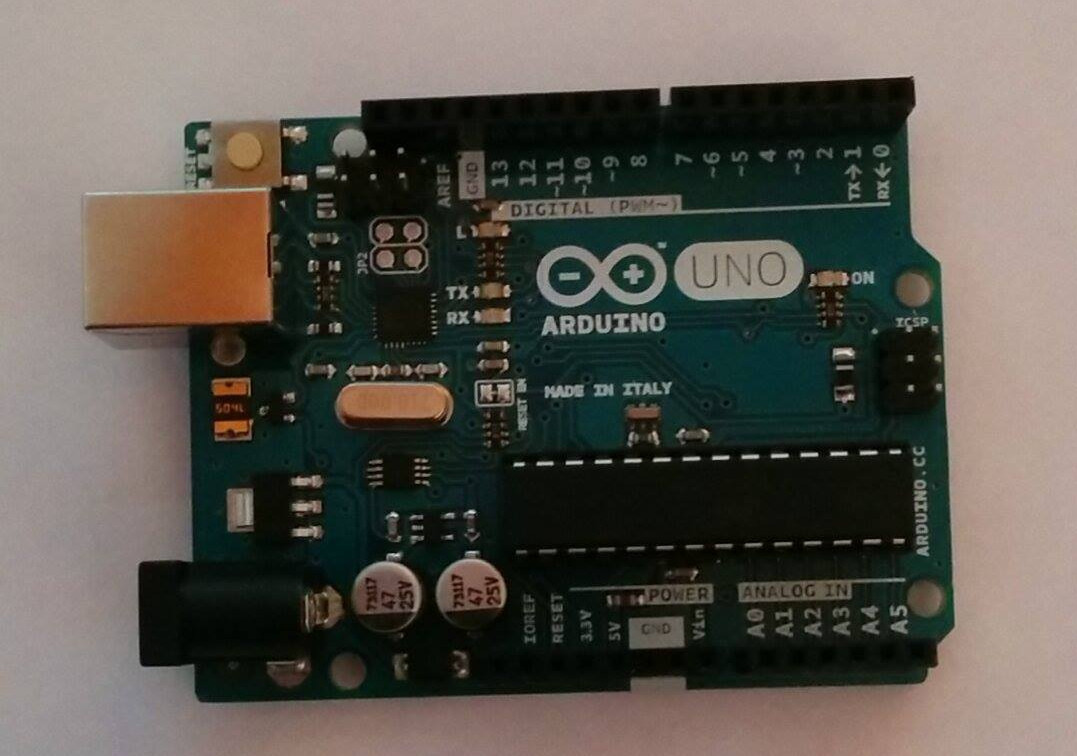
\includegraphics{pic/ardu-uno}}
				\resizebox{0.9\textwidth}{!}{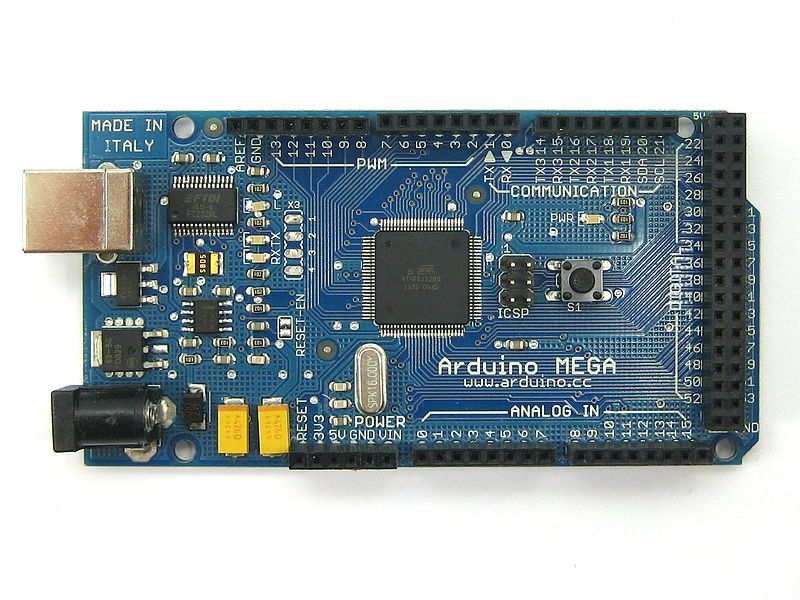
\includegraphics{pic/ardu-mega}}
			\end{column}
		\end{columns}
	\end{frame}

	\begin{frame}[t]{Wires}
		\begin{columns}[T]
			\begin{column}{0.5\textwidth}
				\begin{minipage}{\textwidth}
					\resizebox{0.9\textwidth}{!}{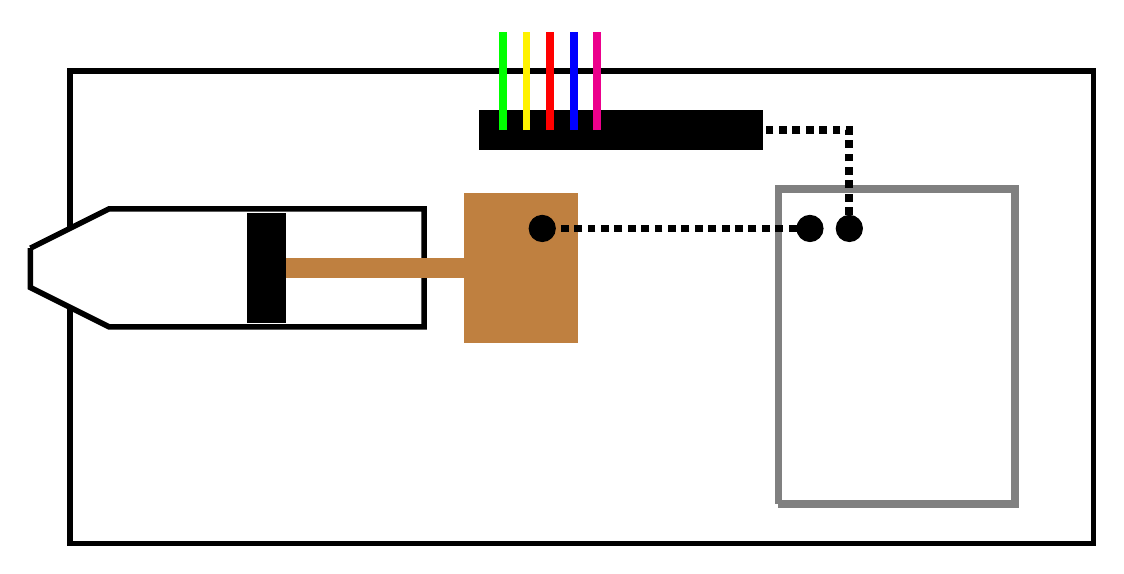
\begin{tikzpicture}
	% Hülle
	\draw[
		line width=0.07cm
	] (1,5) -- (1,2) -- (14,2) -- (14,8) -- (1,8) -- (1,6);
	% Spritze(oben)
	\draw[
		line width=0.07cm
	] (0.5,5.75) -- (0.5,5.25) -- (1.5,4.75) -- (5.5,4.75) -- (5.5,6.25) --
		(1.5,6.25) -- (0.5,5.75);
	% Arduino
	\draw[
		line width=0.1cm,
		color=gray
	] (10,2.5) -- (13,2.5) -- (13,6.5) -- (10,6.5) -- (10,2.5);
	% Servo(oben)
	\draw[
		line width=0.9cm,
		color=brown,
		fill=brown
	] (6,5) -- (7,5) -- (7,6) -- (6,6);
	% Kolben(oben)
	\draw[
		line width=0.5cm,
		color=black
	] (3.5,4.8) -- (3.5,6.2);
	% Verbindung Servo Kolben (oben)
	\draw[
		line width=0.25cm,
		color=brown
	] (3.75,5.5) -- (6,5.5);
	% Ansteuerung Servo (oben)
	\node[
		circle,
		draw,
		fill=black
	] at (10.4,6) {};
	\node[
		circle,
		draw,
		fill=black
	] at (7,6) {};
	\draw[
		dotted,
		color=black,
		line width=0.1cm
	] (10.4,6) -- (7,6);
	% Sensoren-Bank
	\draw[
		fill=black
	] (6.2,7) -- (9.8,7) -- (9.8,7.5) -- (6.2,7.5);
	% Sensoren
	\draw[
		color=green,
		line width=0.1cm
	] (6.5,7.25) -- (6.5,8.5);
	\draw[
		color=yellow,
		line width=0.1cm
	] (6.8,7.25) -- (6.8,8.5);
	\draw[
		color=red,
		line width=0.1cm
	] (7.1,7.25) -- (7.1,8.5);
	\draw[
		color=blue,
		line width=0.1cm
	] (7.4,7.25) -- (7.4,8.5);
	\draw[
		color=magenta,
		line width=0.1cm
	] (7.7,7.25) -- (7.7,8.5);
	% Sensoren Ansteuerung
	\node[
		circle,
		fill=black,
		draw
	] at (10.9,6) {};
	\draw[
		dotted,
		color=black,
		line width=0.1cm
	] (10.9,6) -- (10.9,7.25) -- (9.7,7.25);

\end{tikzpicture}
}
				\end{minipage}
				\begin{minipage}{\textwidth}
					\vspace{0.5cm}
					\begin{itemize}
						\item limited space
						\item power supply for all sensors
						\item[$\Rightarrow$] very monolithic wiring
					\end{itemize}
				\end{minipage}
			\end{column}
			\begin{column}{0.5\textwidth}
				\resizebox{0.9\textwidth}{!}{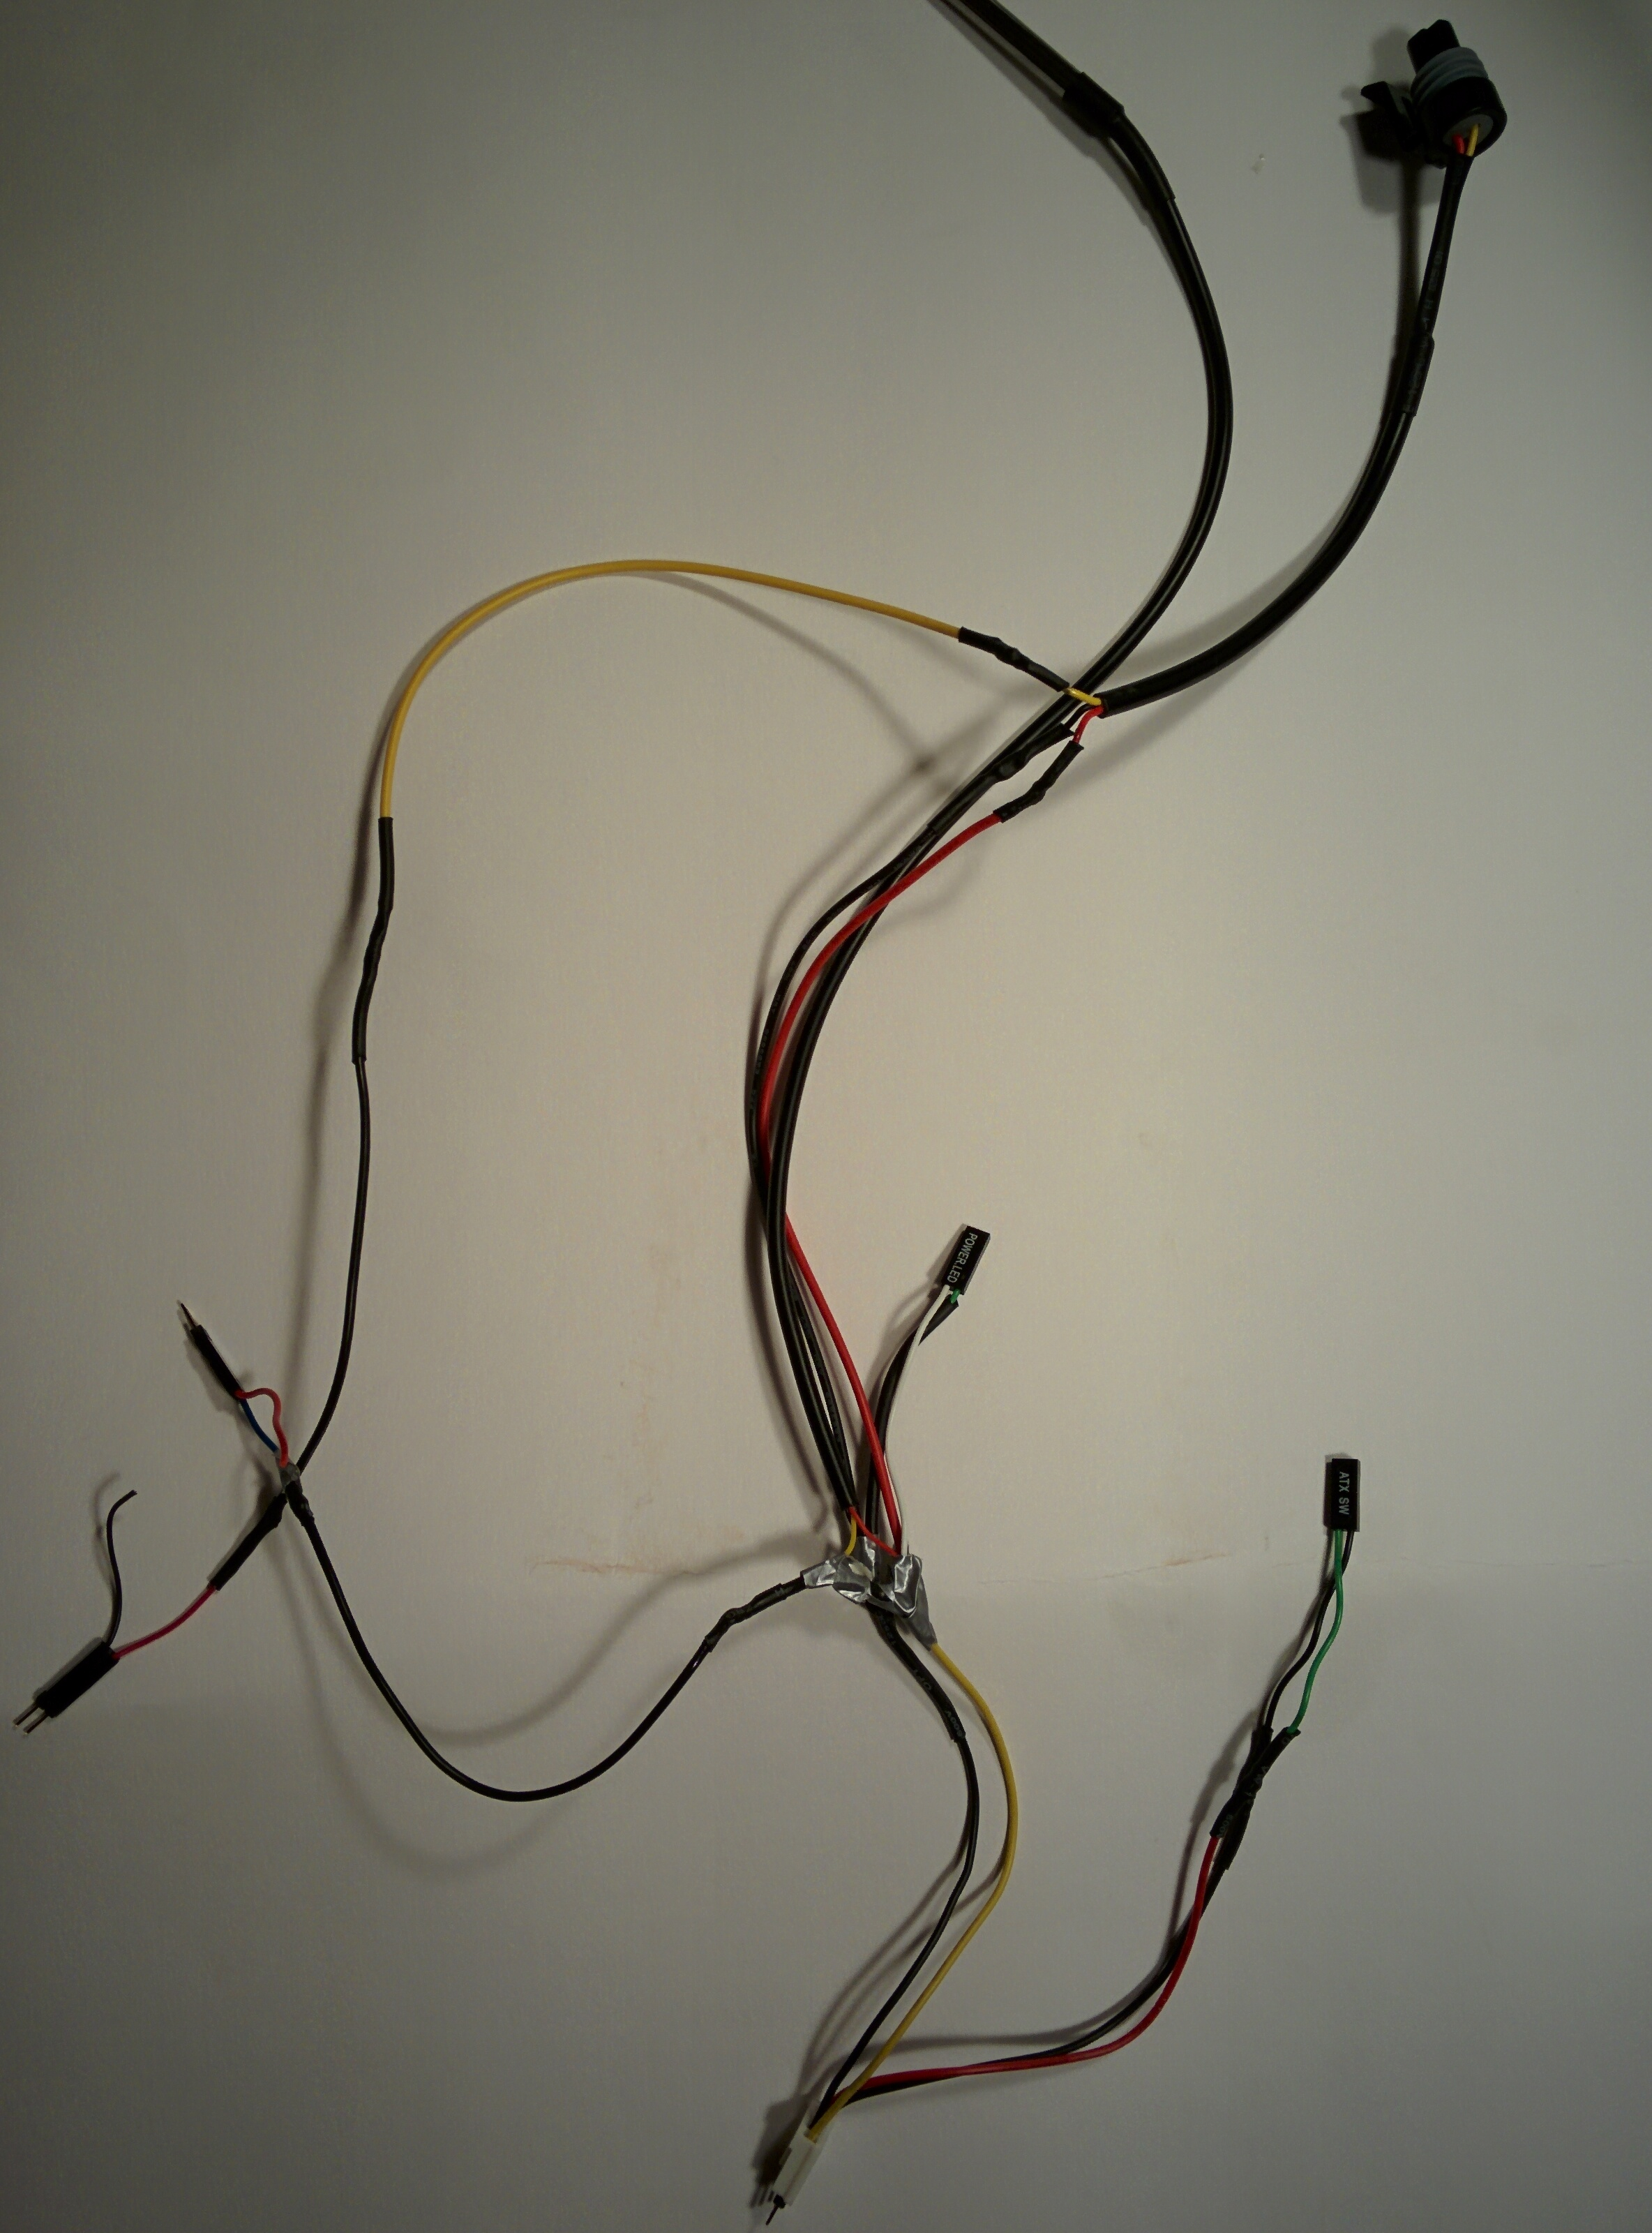
\includegraphics{pic/wires}}
			\end{column}
		\end{columns}
	\end{frame}

	\begin{frame}[t]{Hull}
		\begin{columns}[T]
			\begin{column}{0.5\textwidth}
				\begin{minipage}{\textwidth}
					\resizebox{0.9\textwidth}{!}{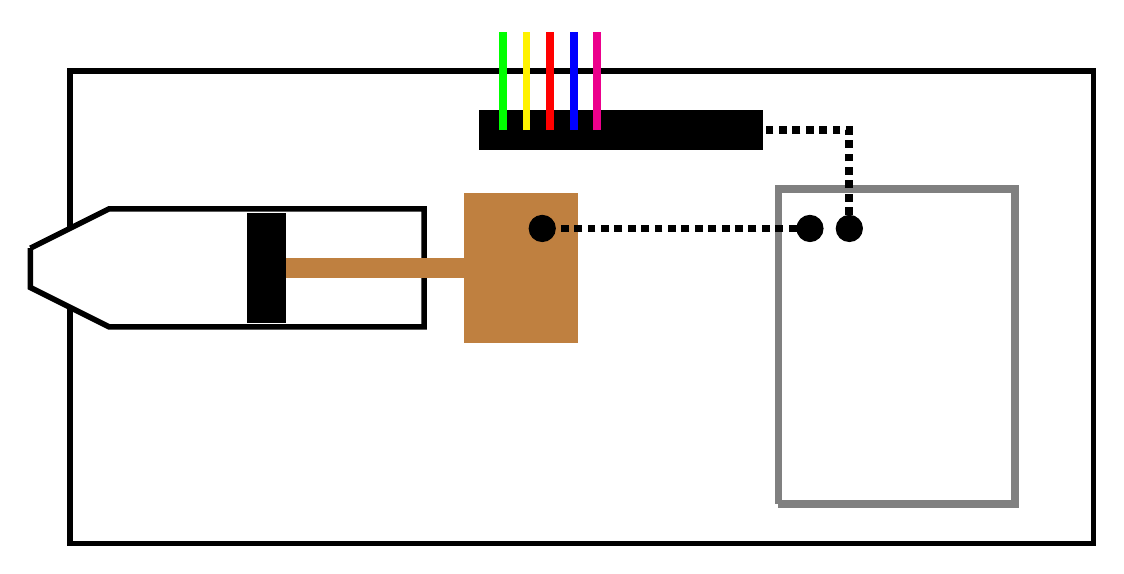
\begin{tikzpicture}
	% Hülle
	\draw[
		line width=0.07cm
	] (1,5) -- (1,2) -- (14,2) -- (14,8) -- (1,8) -- (1,6);
	% Spritze(oben)
	\draw[
		line width=0.07cm
	] (0.5,5.75) -- (0.5,5.25) -- (1.5,4.75) -- (5.5,4.75) -- (5.5,6.25) --
		(1.5,6.25) -- (0.5,5.75);
	% Arduino
	\draw[
		line width=0.1cm,
		color=gray
	] (10,2.5) -- (13,2.5) -- (13,6.5) -- (10,6.5) -- (10,2.5);
	% Servo(oben)
	\draw[
		line width=0.9cm,
		color=brown,
		fill=brown
	] (6,5) -- (7,5) -- (7,6) -- (6,6);
	% Kolben(oben)
	\draw[
		line width=0.5cm,
		color=black
	] (3.5,4.8) -- (3.5,6.2);
	% Verbindung Servo Kolben (oben)
	\draw[
		line width=0.25cm,
		color=brown
	] (3.75,5.5) -- (6,5.5);
	% Ansteuerung Servo (oben)
	\node[
		circle,
		draw,
		fill=black
	] at (10.4,6) {};
	\node[
		circle,
		draw,
		fill=black
	] at (7,6) {};
	\draw[
		dotted,
		color=black,
		line width=0.1cm
	] (10.4,6) -- (7,6);
	% Sensoren-Bank
	\draw[
		fill=black
	] (6.2,7) -- (9.8,7) -- (9.8,7.5) -- (6.2,7.5);
	% Sensoren
	\draw[
		color=green,
		line width=0.1cm
	] (6.5,7.25) -- (6.5,8.5);
	\draw[
		color=yellow,
		line width=0.1cm
	] (6.8,7.25) -- (6.8,8.5);
	\draw[
		color=red,
		line width=0.1cm
	] (7.1,7.25) -- (7.1,8.5);
	\draw[
		color=blue,
		line width=0.1cm
	] (7.4,7.25) -- (7.4,8.5);
	\draw[
		color=magenta,
		line width=0.1cm
	] (7.7,7.25) -- (7.7,8.5);
	% Sensoren Ansteuerung
	\node[
		circle,
		fill=black,
		draw
	] at (10.9,6) {};
	\draw[
		dotted,
		color=black,
		line width=0.1cm
	] (10.9,6) -- (10.9,7.25) -- (9.7,7.25);

\end{tikzpicture}
}
				\end{minipage}
				\begin{minipage}{\textwidth}
					\vspace{0.5cm}
					\begin{itemize}
						\item PVC pipe
						\item commonly used for fluids
							\begin{itemize}
								\item modular
								\item equipped with seals
								\item leakproof
							\end{itemize}
					\end{itemize}
				\end{minipage}
			\end{column}
			\begin{column}{0.5\textwidth}
				\begin{center}
					\resizebox{0.3\textwidth}{!}{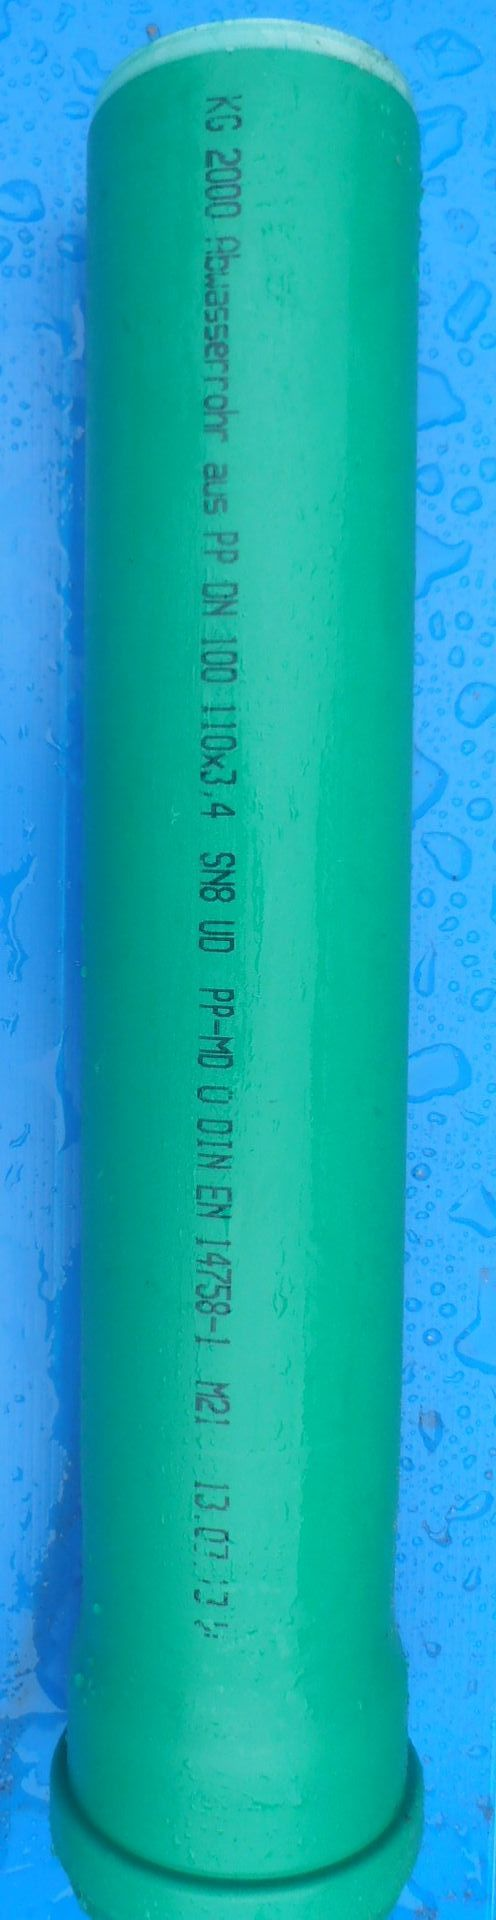
\includegraphics{pic/pvchull}}
				\end{center}
			\end{column}
		\end{columns}
	\end{frame}

	\begin{frame}{Challenges}
		\begin{columns}
			\column{0.5\textwidth}
				\begin{itemize}
					\item capacity of diving tank
						\begin{itemize}
							\item around 3\% of actual volume
							\item[$\Rightarrow$] very difficult to tare
						\end{itemize}
				\end{itemize}
			\column{0.5\textwidth}
				\begin{itemize}
					\item construction of diving tank
						\begin{itemize}
							\item leakproof all moving parts
						\end{itemize}
					\item permanently attach things to PVC hull
					\item leakproof all outgoing parts
				\end{itemize}
		\end{columns}
	\end{frame}
	
	\begin{frame}{Expenses}
		\begin{center}
			\begin{tabular}{|lr|}
				\hline
				Item & Expenses \\\hline
				PVC Hull & \euro{10}\\
				Stepper & \euro{20}\\
				Threaded Rod, Wave-Coupling, Nuts & \euro{10}\\
				Stepper Driver & \euro{ 4}\\
				Arduino Mega & \euro{20}\\\hline
				$\Sigma$ & \euro{54}\\
				\hline
			\end{tabular}
		\end{center}
	\end{frame}

	\section{Future Ideas}
	\begin{frame}{Future Ideas}
		\begin{columns}
			\column{0.5\textwidth}
			\begin{itemize}
				\item modularize
					\begin{itemize}
						\item communication topology for sensors
						\item power bus for sensors
					\end{itemize}
				\item underwater sensor networks
					\begin{itemize}
						\item under-water communication
						\item measuring boxes
					\end{itemize}
			\end{itemize}
			\column{0.5\textwidth}
			\begin{itemize}
				\item autonomize
					\begin{itemize}
						\item wireless charging
						\item wireless software updates
						\item common interface to add sensors in self containing hulls
					\end{itemize}
				\item add drive
			\end{itemize}
		\end{columns}
		\begin{mdframed}
			\begin{center}
				Keep up with the submarine project on\\
				http://voltidioten.westhofen.info/
			\end{center}
		\end{mdframed}
		\let\thefootnote\relax\footnote{further reference: https://hackaday.io/list/7359-waterborne-projects}
	\end{frame}

	\begin{frame}{Acknowledgments}
		\begin{center}
			We want to thank some fellow submarine constructors, namely:
		\end{center}
		\begin{itemize}
			\item Thomas Welzel
			\item Martin Welzel
			\item Winfried Harking
		\end{itemize}
	\end{frame}

\end{document}
